\documentclass[twoside]{book}

% Packages required by doxygen
\usepackage{fixltx2e}
\usepackage{calc}
\usepackage{doxygen}
\usepackage[export]{adjustbox} % also loads graphicx
\usepackage{graphicx}
\usepackage[utf8]{inputenc}
\usepackage{makeidx}
\usepackage{multicol}
\usepackage{multirow}
\PassOptionsToPackage{warn}{textcomp}
\usepackage{textcomp}
\usepackage[nointegrals]{wasysym}
\usepackage[table]{xcolor}

% Font selection
\usepackage[T1]{fontenc}
\usepackage[scaled=.90]{helvet}
\usepackage{courier}
\usepackage{amssymb}
\usepackage{sectsty}
\renewcommand{\familydefault}{\sfdefault}
\allsectionsfont{%
  \fontseries{bc}\selectfont%
  \color{darkgray}%
}
\renewcommand{\DoxyLabelFont}{%
  \fontseries{bc}\selectfont%
  \color{darkgray}%
}
\newcommand{\+}{\discretionary{\mbox{\scriptsize$\hookleftarrow$}}{}{}}

% Page & text layout
\usepackage{geometry}
\geometry{%
  a4paper,%
  top=2.5cm,%
  bottom=2.5cm,%
  left=2.5cm,%
  right=2.5cm%
}
\tolerance=750
\hfuzz=15pt
\hbadness=750
\setlength{\emergencystretch}{15pt}
\setlength{\parindent}{0cm}
\setlength{\parskip}{3ex plus 2ex minus 2ex}
\makeatletter
\renewcommand{\paragraph}{%
  \@startsection{paragraph}{4}{0ex}{-1.0ex}{1.0ex}{%
    \normalfont\normalsize\bfseries\SS@parafont%
  }%
}
\renewcommand{\subparagraph}{%
  \@startsection{subparagraph}{5}{0ex}{-1.0ex}{1.0ex}{%
    \normalfont\normalsize\bfseries\SS@subparafont%
  }%
}
\makeatother

% Headers & footers
\usepackage{fancyhdr}
\pagestyle{fancyplain}
\fancyhead[LE]{\fancyplain{}{\bfseries\thepage}}
\fancyhead[CE]{\fancyplain{}{}}
\fancyhead[RE]{\fancyplain{}{\bfseries\leftmark}}
\fancyhead[LO]{\fancyplain{}{\bfseries\rightmark}}
\fancyhead[CO]{\fancyplain{}{}}
\fancyhead[RO]{\fancyplain{}{\bfseries\thepage}}
\fancyfoot[LE]{\fancyplain{}{}}
\fancyfoot[CE]{\fancyplain{}{}}
\fancyfoot[RE]{\fancyplain{}{\bfseries\scriptsize Generated by Doxygen }}
\fancyfoot[LO]{\fancyplain{}{\bfseries\scriptsize Generated by Doxygen }}
\fancyfoot[CO]{\fancyplain{}{}}
\fancyfoot[RO]{\fancyplain{}{}}
\renewcommand{\footrulewidth}{0.4pt}
\renewcommand{\chaptermark}[1]{%
  \markboth{#1}{}%
}
\renewcommand{\sectionmark}[1]{%
  \markright{\thesection\ #1}%
}

% Indices & bibliography
\usepackage{natbib}
\usepackage[titles]{tocloft}
\setcounter{tocdepth}{3}
\setcounter{secnumdepth}{5}
\makeindex

% Hyperlinks (required, but should be loaded last)
\usepackage{ifpdf}
\ifpdf
  \usepackage[pdftex,pagebackref=true]{hyperref}
\else
  \usepackage[ps2pdf,pagebackref=true]{hyperref}
\fi
\hypersetup{%
  colorlinks=true,%
  linkcolor=blue,%
  citecolor=blue,%
  unicode%
}

% Custom commands
\newcommand{\clearemptydoublepage}{%
  \newpage{\pagestyle{empty}\cleardoublepage}%
}

\usepackage{caption}
\captionsetup{labelsep=space,justification=centering,font={bf},singlelinecheck=off,skip=4pt,position=top}

%===== C O N T E N T S =====

\begin{document}

% Titlepage & ToC
\hypersetup{pageanchor=false,
             bookmarksnumbered=true,
             pdfencoding=unicode
            }
\pagenumbering{alph}
\begin{titlepage}
\vspace*{7cm}
\begin{center}%
{\Large data-\/juggler }\\
\vspace*{1cm}
{\large Generated by Doxygen 1.8.13}\\
\end{center}
\end{titlepage}
\clearemptydoublepage
\pagenumbering{roman}
\tableofcontents
\clearemptydoublepage
\pagenumbering{arabic}
\hypersetup{pageanchor=true}

%--- Begin generated contents ---
\chapter{data-\/juggler}
\label{index}\hypertarget{index}{}This is a set of portable C++ codes that perform optimized data organization features such as item collections (lists and trees), strings, among other things. This library is under development and does not have enough descriptive documents. Look at the source code itself to better understand its operation.

\subsection*{How to include this in my code}

To use this library in your C ++ program, you must include the datajuggler.\+hpp header in your code. When compiling your program, you should give all .o files from the obj directory or all .cpp files from the src directory to the compiler to compile the datajuggler together with your program. 
\chapter{Hierarchical Index}
\section{Class Hierarchy}
This inheritance list is sorted roughly, but not completely, alphabetically\+:\begin{DoxyCompactList}
\item \contentsline{section}{Data\+Juggler\+:\+:Binary\+Tree\+Node}{\pageref{classDataJuggler_1_1BinaryTreeNode}}{}
\item \contentsline{section}{Data\+Juggler\+:\+:Exception}{\pageref{classDataJuggler_1_1Exception}}{}
\begin{DoxyCompactList}
\item \contentsline{section}{Data\+Juggler\+:\+:Damaged\+Linked\+List\+Ex}{\pageref{classDataJuggler_1_1DamagedLinkedListEx}}{}
\item \contentsline{section}{Data\+Juggler\+:\+:Invalid\+Args\+Ex}{\pageref{classDataJuggler_1_1InvalidArgsEx}}{}
\item \contentsline{section}{Data\+Juggler\+:\+:String\+Hash\+Out\+Of\+Set\+Ex}{\pageref{classDataJuggler_1_1StringHashOutOfSetEx}}{}
\item \contentsline{section}{Data\+Juggler\+:\+:String\+Hash\+Overflow\+Ex}{\pageref{classDataJuggler_1_1StringHashOverflowEx}}{}
\end{DoxyCompactList}
\item \contentsline{section}{Data\+Juggler\+:\+:Linked\+List\+Node\+:\+:Header}{\pageref{classDataJuggler_1_1LinkedListNode_1_1Header}}{}
\item \contentsline{section}{Data\+Juggler\+:\+:Linked\+List\+Node}{\pageref{classDataJuggler_1_1LinkedListNode}}{}
\end{DoxyCompactList}

\chapter{Class Index}
\section{Class List}
Here are the classes, structs, unions and interfaces with brief descriptions\+:\begin{DoxyCompactList}
\item\contentsline{section}{\hyperlink{classDataJuggler_1_1BinaryTreeNode}{Data\+Juggler\+::\+Binary\+Tree\+Node} }{\pageref{classDataJuggler_1_1BinaryTreeNode}}{}
\item\contentsline{section}{\hyperlink{classDataJuggler_1_1DamagedLinkedListEx}{Data\+Juggler\+::\+Damaged\+Linked\+List\+Ex} }{\pageref{classDataJuggler_1_1DamagedLinkedListEx}}{}
\item\contentsline{section}{\hyperlink{classDataJuggler_1_1Exception}{Data\+Juggler\+::\+Exception} }{\pageref{classDataJuggler_1_1Exception}}{}
\item\contentsline{section}{\hyperlink{classDataJuggler_1_1LinkedListNode_1_1Header}{Data\+Juggler\+::\+Linked\+List\+Node\+::\+Header} }{\pageref{classDataJuggler_1_1LinkedListNode_1_1Header}}{}
\item\contentsline{section}{\hyperlink{classDataJuggler_1_1InvalidArgsEx}{Data\+Juggler\+::\+Invalid\+Args\+Ex} }{\pageref{classDataJuggler_1_1InvalidArgsEx}}{}
\item\contentsline{section}{\hyperlink{classDataJuggler_1_1LinkedListNode}{Data\+Juggler\+::\+Linked\+List\+Node} }{\pageref{classDataJuggler_1_1LinkedListNode}}{}
\item\contentsline{section}{\hyperlink{classDataJuggler_1_1StringHashOutOfSetEx}{Data\+Juggler\+::\+String\+Hash\+Out\+Of\+Set\+Ex} }{\pageref{classDataJuggler_1_1StringHashOutOfSetEx}}{}
\item\contentsline{section}{\hyperlink{classDataJuggler_1_1StringHashOverflowEx}{Data\+Juggler\+::\+String\+Hash\+Overflow\+Ex} }{\pageref{classDataJuggler_1_1StringHashOverflowEx}}{}
\end{DoxyCompactList}

\chapter{Class Documentation}
\hypertarget{classDataJuggler_1_1BinaryTreeNode}{}\section{Data\+Juggler\+:\+:Binary\+Tree\+Node Class Reference}
\label{classDataJuggler_1_1BinaryTreeNode}\index{Data\+Juggler\+::\+Binary\+Tree\+Node@{Data\+Juggler\+::\+Binary\+Tree\+Node}}


{\ttfamily \#include $<$treenode.\+hpp$>$}



Collaboration diagram for Data\+Juggler\+:\+:Binary\+Tree\+Node\+:\nopagebreak
\begin{figure}[H]
\begin{center}
\leavevmode
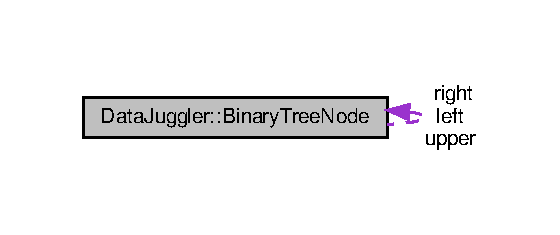
\includegraphics[width=269pt]{classDataJuggler_1_1BinaryTreeNode__coll__graph}
\end{center}
\end{figure}
\subsection*{Public Types}
\begin{DoxyCompactItemize}
\item 
\mbox{\Hypertarget{classDataJuggler_1_1BinaryTreeNode_a3fefd287cd17d15b5905296826eca754}\label{classDataJuggler_1_1BinaryTreeNode_a3fefd287cd17d15b5905296826eca754}} 
enum {\bfseries Branch} \{ {\bfseries left\+\_\+branch}, 
{\bfseries right\+\_\+branch}, 
{\bfseries none\+\_\+branch}
 \}
\end{DoxyCompactItemize}
\subsection*{Public Member Functions}
\begin{DoxyCompactItemize}
\item 
virtual \hyperlink{classDataJuggler_1_1BinaryTreeNode_af2995ef47057ef14f617af026998afc1}{$\sim$\+Binary\+Tree\+Node} ()
\item 
void \hyperlink{classDataJuggler_1_1BinaryTreeNode_a39df9c1d2ae67bb35323548e83601bd4}{pre\+Order} (function$<$ void(\hyperlink{classDataJuggler_1_1BinaryTreeNode}{Binary\+Tree\+Node} $\ast$)$>$ callback)
\item 
void \hyperlink{classDataJuggler_1_1BinaryTreeNode_a082f4223f8d7d40c5e85a9f2322a2b22}{symmetrical\+Order} (function$<$ void(\hyperlink{classDataJuggler_1_1BinaryTreeNode}{Binary\+Tree\+Node} $\ast$)$>$ callback)
\item 
void \hyperlink{classDataJuggler_1_1BinaryTreeNode_ad52d331c7d393615f76bb18657dc7c0b}{post\+Order} (function$<$ void(\hyperlink{classDataJuggler_1_1BinaryTreeNode}{Binary\+Tree\+Node} $\ast$)$>$ callback)
\item 
void \hyperlink{classDataJuggler_1_1BinaryTreeNode_a65f216d77e7953f02dfa4bc293fd8993}{insert\+Left} (\hyperlink{classDataJuggler_1_1BinaryTreeNode}{Binary\+Tree\+Node} $\ast$to\+\_\+insert)
\item 
void \hyperlink{classDataJuggler_1_1BinaryTreeNode_ac59067ab56902eafb5b7c541276c294c}{insert\+Right} (\hyperlink{classDataJuggler_1_1BinaryTreeNode}{Binary\+Tree\+Node} $\ast$to\+\_\+insert)
\item 
Branch \hyperlink{classDataJuggler_1_1BinaryTreeNode_a98ff5ed818a8a679979adaae76fcbd8a}{get\+Branch\+Of\+Upper} ()
\item 
\hyperlink{classDataJuggler_1_1BinaryTreeNode}{Binary\+Tree\+Node} $\ast$ \hyperlink{classDataJuggler_1_1BinaryTreeNode_a07f3536b32e66d434b426f2d4903710a}{get\+Upper} ()
\item 
\hyperlink{classDataJuggler_1_1BinaryTreeNode}{Binary\+Tree\+Node} $\ast$ \hyperlink{classDataJuggler_1_1BinaryTreeNode_a9c7bf23457f5a2a39a6b7e5525604e68}{get\+Left} ()
\item 
\hyperlink{classDataJuggler_1_1BinaryTreeNode}{Binary\+Tree\+Node} $\ast$ \hyperlink{classDataJuggler_1_1BinaryTreeNode_a0d7d9c5d8cd5033e12f78dfbcb9667a1}{get\+Right} ()
\item 
\hyperlink{classDataJuggler_1_1BinaryTreeNode}{Binary\+Tree\+Node} $\ast$ \hyperlink{classDataJuggler_1_1BinaryTreeNode_a257b78d609886933af1ceabb8c5880b0}{get\+Supertree\+Root} ()
\item 
\hyperlink{classDataJuggler_1_1BinaryTreeNode}{Binary\+Tree\+Node} $\ast$ \hyperlink{classDataJuggler_1_1BinaryTreeNode_a7e0d717313cf4ca8fe28e9663dd2c299}{get\+Deeper\+Subtree\+Leaf} ()
\item 
long \hyperlink{classDataJuggler_1_1BinaryTreeNode_a0ee7e550e37a7882e5bab3be3fac1a42}{get\+Distance\+To} (\hyperlink{classDataJuggler_1_1BinaryTreeNode}{Binary\+Tree\+Node} $\ast$reference)
\item 
bool \hyperlink{classDataJuggler_1_1BinaryTreeNode_a51c9d0cc830439528546be1d2c42ce72}{is\+Root} ()
\item 
bool \hyperlink{classDataJuggler_1_1BinaryTreeNode_a6716143fcaf85866773b85f3342114d9}{is\+Leaf} ()
\item 
bool \hyperlink{classDataJuggler_1_1BinaryTreeNode_a2ca8921083f09fdc947bfc8be1af834a}{is\+Only} ()
\item 
virtual void \hyperlink{classDataJuggler_1_1BinaryTreeNode_a563663d605400e2a928df19fd086bf9a}{delete\+Subtree} ()
\end{DoxyCompactItemize}
\subsection*{Static Protected Member Functions}
\begin{DoxyCompactItemize}
\item 
\mbox{\Hypertarget{classDataJuggler_1_1BinaryTreeNode_a6c7ea66bec6d5371e4a065b859f53939}\label{classDataJuggler_1_1BinaryTreeNode_a6c7ea66bec6d5371e4a065b859f53939}} 
static long {\bfseries recursive\+Get\+Distance\+Down} (\hyperlink{classDataJuggler_1_1BinaryTreeNode}{Binary\+Tree\+Node} $\ast$from, \hyperlink{classDataJuggler_1_1BinaryTreeNode}{Binary\+Tree\+Node} $\ast$to, long counter=1)
\end{DoxyCompactItemize}
\subsection*{Protected Attributes}
\begin{DoxyCompactItemize}
\item 
\mbox{\Hypertarget{classDataJuggler_1_1BinaryTreeNode_ac4fc27cfb417375f9b9867f52ec03019}\label{classDataJuggler_1_1BinaryTreeNode_ac4fc27cfb417375f9b9867f52ec03019}} 
Branch {\bfseries on\+Branch\+Of\+Upper}
\item 
\mbox{\Hypertarget{classDataJuggler_1_1BinaryTreeNode_a731d7b7e81097ea2d3173717ad272c5f}\label{classDataJuggler_1_1BinaryTreeNode_a731d7b7e81097ea2d3173717ad272c5f}} 
\hyperlink{classDataJuggler_1_1BinaryTreeNode}{Binary\+Tree\+Node} $\ast$ {\bfseries upper}
\item 
\mbox{\Hypertarget{classDataJuggler_1_1BinaryTreeNode_a1ea539098abf8cbcb5afdffa9061f2df}\label{classDataJuggler_1_1BinaryTreeNode_a1ea539098abf8cbcb5afdffa9061f2df}} 
\hyperlink{classDataJuggler_1_1BinaryTreeNode}{Binary\+Tree\+Node} $\ast$ {\bfseries left}
\item 
\mbox{\Hypertarget{classDataJuggler_1_1BinaryTreeNode_a874efcd449929ca1ac8c881c93621a7f}\label{classDataJuggler_1_1BinaryTreeNode_a874efcd449929ca1ac8c881c93621a7f}} 
\hyperlink{classDataJuggler_1_1BinaryTreeNode}{Binary\+Tree\+Node} $\ast$ {\bfseries right}
\end{DoxyCompactItemize}


\subsection{Detailed Description}
This class represents the node of a binary tree, with pointer to left branch, direct branch, and upper node. This class is very basic and should not be instantiated directly. Subclasses of this can be used to enter information (such as numbers, keys, objects) on the node and perform operations such as rotation and sorting on the tree. 

\subsection{Constructor \& Destructor Documentation}
\mbox{\Hypertarget{classDataJuggler_1_1BinaryTreeNode_af2995ef47057ef14f617af026998afc1}\label{classDataJuggler_1_1BinaryTreeNode_af2995ef47057ef14f617af026998afc1}} 
\index{Data\+Juggler\+::\+Binary\+Tree\+Node@{Data\+Juggler\+::\+Binary\+Tree\+Node}!````~Binary\+Tree\+Node@{$\sim$\+Binary\+Tree\+Node}}
\index{````~Binary\+Tree\+Node@{$\sim$\+Binary\+Tree\+Node}!Data\+Juggler\+::\+Binary\+Tree\+Node@{Data\+Juggler\+::\+Binary\+Tree\+Node}}
\subsubsection{\texorpdfstring{$\sim$\+Binary\+Tree\+Node()}{~BinaryTreeNode()}}
{\footnotesize\ttfamily Data\+Juggler\+::\+Binary\+Tree\+Node\+::$\sim$\+Binary\+Tree\+Node (\begin{DoxyParamCaption}{ }\end{DoxyParamCaption})\hspace{0.3cm}{\ttfamily [virtual]}}

this destructor assign nullptr to all references to this \hyperlink{classDataJuggler_1_1BinaryTreeNode}{Binary\+Tree\+Node} in the supertree in which it is inserted. Use very carefully, as the rest of the subtree is not deleted, maying cause a memory leakage. To delete the entire subtree, use the delete\+Subtree function of the same class. 

\subsection{Member Function Documentation}
\mbox{\Hypertarget{classDataJuggler_1_1BinaryTreeNode_a563663d605400e2a928df19fd086bf9a}\label{classDataJuggler_1_1BinaryTreeNode_a563663d605400e2a928df19fd086bf9a}} 
\index{Data\+Juggler\+::\+Binary\+Tree\+Node@{Data\+Juggler\+::\+Binary\+Tree\+Node}!delete\+Subtree@{delete\+Subtree}}
\index{delete\+Subtree@{delete\+Subtree}!Data\+Juggler\+::\+Binary\+Tree\+Node@{Data\+Juggler\+::\+Binary\+Tree\+Node}}
\subsubsection{\texorpdfstring{delete\+Subtree()}{deleteSubtree()}}
{\footnotesize\ttfamily void Data\+Juggler\+::\+Binary\+Tree\+Node\+::delete\+Subtree (\begin{DoxyParamCaption}{ }\end{DoxyParamCaption})\hspace{0.3cm}{\ttfamily [virtual]}}

This function recursively deletes all Binary\+Tree\+Nodes from the subtree of which this is the root. I\+M\+P\+O\+R\+T\+A\+NT\+: After using this function, it is not necessary to use the destructor of this class to delete this \hyperlink{classDataJuggler_1_1BinaryTreeNode}{Binary\+Tree\+Node} as this will cause a segmentation fault. \mbox{\Hypertarget{classDataJuggler_1_1BinaryTreeNode_a98ff5ed818a8a679979adaae76fcbd8a}\label{classDataJuggler_1_1BinaryTreeNode_a98ff5ed818a8a679979adaae76fcbd8a}} 
\index{Data\+Juggler\+::\+Binary\+Tree\+Node@{Data\+Juggler\+::\+Binary\+Tree\+Node}!get\+Branch\+Of\+Upper@{get\+Branch\+Of\+Upper}}
\index{get\+Branch\+Of\+Upper@{get\+Branch\+Of\+Upper}!Data\+Juggler\+::\+Binary\+Tree\+Node@{Data\+Juggler\+::\+Binary\+Tree\+Node}}
\subsubsection{\texorpdfstring{get\+Branch\+Of\+Upper()}{getBranchOfUpper()}}
{\footnotesize\ttfamily Binary\+Tree\+Node\+::\+Branch Data\+Juggler\+::\+Binary\+Tree\+Node\+::get\+Branch\+Of\+Upper (\begin{DoxyParamCaption}{ }\end{DoxyParamCaption})}

This function returns an information of type Binary\+Tree\+Node\+::\+Branch informing which of the two branches (left or right) of the upper \hyperlink{classDataJuggler_1_1BinaryTreeNode}{Binary\+Tree\+Node} this \hyperlink{classDataJuggler_1_1BinaryTreeNode}{Binary\+Tree\+Node} has been inserted. \mbox{\Hypertarget{classDataJuggler_1_1BinaryTreeNode_a7e0d717313cf4ca8fe28e9663dd2c299}\label{classDataJuggler_1_1BinaryTreeNode_a7e0d717313cf4ca8fe28e9663dd2c299}} 
\index{Data\+Juggler\+::\+Binary\+Tree\+Node@{Data\+Juggler\+::\+Binary\+Tree\+Node}!get\+Deeper\+Subtree\+Leaf@{get\+Deeper\+Subtree\+Leaf}}
\index{get\+Deeper\+Subtree\+Leaf@{get\+Deeper\+Subtree\+Leaf}!Data\+Juggler\+::\+Binary\+Tree\+Node@{Data\+Juggler\+::\+Binary\+Tree\+Node}}
\subsubsection{\texorpdfstring{get\+Deeper\+Subtree\+Leaf()}{getDeeperSubtreeLeaf()}}
{\footnotesize\ttfamily \hyperlink{classDataJuggler_1_1BinaryTreeNode}{Binary\+Tree\+Node} $\ast$ Data\+Juggler\+::\+Binary\+Tree\+Node\+::get\+Deeper\+Subtree\+Leaf (\begin{DoxyParamCaption}{ }\end{DoxyParamCaption})}

This function fetches the deepest \hyperlink{classDataJuggler_1_1BinaryTreeNode}{Binary\+Tree\+Node} in the tree whose root is this. \mbox{\Hypertarget{classDataJuggler_1_1BinaryTreeNode_a0ee7e550e37a7882e5bab3be3fac1a42}\label{classDataJuggler_1_1BinaryTreeNode_a0ee7e550e37a7882e5bab3be3fac1a42}} 
\index{Data\+Juggler\+::\+Binary\+Tree\+Node@{Data\+Juggler\+::\+Binary\+Tree\+Node}!get\+Distance\+To@{get\+Distance\+To}}
\index{get\+Distance\+To@{get\+Distance\+To}!Data\+Juggler\+::\+Binary\+Tree\+Node@{Data\+Juggler\+::\+Binary\+Tree\+Node}}
\subsubsection{\texorpdfstring{get\+Distance\+To()}{getDistanceTo()}}
{\footnotesize\ttfamily long Data\+Juggler\+::\+Binary\+Tree\+Node\+::get\+Distance\+To (\begin{DoxyParamCaption}\item[{\hyperlink{classDataJuggler_1_1BinaryTreeNode}{Binary\+Tree\+Node} $\ast$}]{reference }\end{DoxyParamCaption})}

This function obtains the distance of this \hyperlink{classDataJuggler_1_1BinaryTreeNode}{Binary\+Tree\+Node} to another \hyperlink{classDataJuggler_1_1BinaryTreeNode}{Binary\+Tree\+Node} of the same supertree (which must be passed as argument of this function). If the \hyperlink{classDataJuggler_1_1BinaryTreeNode}{Binary\+Tree\+Node} passed as argument is not part of the same tree as this, the function returns -\/1. \mbox{\Hypertarget{classDataJuggler_1_1BinaryTreeNode_a9c7bf23457f5a2a39a6b7e5525604e68}\label{classDataJuggler_1_1BinaryTreeNode_a9c7bf23457f5a2a39a6b7e5525604e68}} 
\index{Data\+Juggler\+::\+Binary\+Tree\+Node@{Data\+Juggler\+::\+Binary\+Tree\+Node}!get\+Left@{get\+Left}}
\index{get\+Left@{get\+Left}!Data\+Juggler\+::\+Binary\+Tree\+Node@{Data\+Juggler\+::\+Binary\+Tree\+Node}}
\subsubsection{\texorpdfstring{get\+Left()}{getLeft()}}
{\footnotesize\ttfamily \hyperlink{classDataJuggler_1_1BinaryTreeNode}{Binary\+Tree\+Node} $\ast$ Data\+Juggler\+::\+Binary\+Tree\+Node\+::get\+Left (\begin{DoxyParamCaption}{ }\end{DoxyParamCaption})}

This function gets a pointer to the \hyperlink{classDataJuggler_1_1BinaryTreeNode}{Binary\+Tree\+Node} on the left branch from this \hyperlink{classDataJuggler_1_1BinaryTreeNode}{Binary\+Tree\+Node} \mbox{\Hypertarget{classDataJuggler_1_1BinaryTreeNode_a0d7d9c5d8cd5033e12f78dfbcb9667a1}\label{classDataJuggler_1_1BinaryTreeNode_a0d7d9c5d8cd5033e12f78dfbcb9667a1}} 
\index{Data\+Juggler\+::\+Binary\+Tree\+Node@{Data\+Juggler\+::\+Binary\+Tree\+Node}!get\+Right@{get\+Right}}
\index{get\+Right@{get\+Right}!Data\+Juggler\+::\+Binary\+Tree\+Node@{Data\+Juggler\+::\+Binary\+Tree\+Node}}
\subsubsection{\texorpdfstring{get\+Right()}{getRight()}}
{\footnotesize\ttfamily \hyperlink{classDataJuggler_1_1BinaryTreeNode}{Binary\+Tree\+Node} $\ast$ Data\+Juggler\+::\+Binary\+Tree\+Node\+::get\+Right (\begin{DoxyParamCaption}{ }\end{DoxyParamCaption})}

This function gets a pointer to the \hyperlink{classDataJuggler_1_1BinaryTreeNode}{Binary\+Tree\+Node} on the right branch from this \hyperlink{classDataJuggler_1_1BinaryTreeNode}{Binary\+Tree\+Node} \mbox{\Hypertarget{classDataJuggler_1_1BinaryTreeNode_a257b78d609886933af1ceabb8c5880b0}\label{classDataJuggler_1_1BinaryTreeNode_a257b78d609886933af1ceabb8c5880b0}} 
\index{Data\+Juggler\+::\+Binary\+Tree\+Node@{Data\+Juggler\+::\+Binary\+Tree\+Node}!get\+Supertree\+Root@{get\+Supertree\+Root}}
\index{get\+Supertree\+Root@{get\+Supertree\+Root}!Data\+Juggler\+::\+Binary\+Tree\+Node@{Data\+Juggler\+::\+Binary\+Tree\+Node}}
\subsubsection{\texorpdfstring{get\+Supertree\+Root()}{getSupertreeRoot()}}
{\footnotesize\ttfamily \hyperlink{classDataJuggler_1_1BinaryTreeNode}{Binary\+Tree\+Node} $\ast$ Data\+Juggler\+::\+Binary\+Tree\+Node\+::get\+Supertree\+Root (\begin{DoxyParamCaption}{ }\end{DoxyParamCaption})}

This function gets the root of the supertree on which this \hyperlink{classDataJuggler_1_1BinaryTreeNode}{Binary\+Tree\+Node} is inserted. If this \hyperlink{classDataJuggler_1_1BinaryTreeNode}{Binary\+Tree\+Node} is the root of the tree itself, this function returns a pointer to it same. \mbox{\Hypertarget{classDataJuggler_1_1BinaryTreeNode_a07f3536b32e66d434b426f2d4903710a}\label{classDataJuggler_1_1BinaryTreeNode_a07f3536b32e66d434b426f2d4903710a}} 
\index{Data\+Juggler\+::\+Binary\+Tree\+Node@{Data\+Juggler\+::\+Binary\+Tree\+Node}!get\+Upper@{get\+Upper}}
\index{get\+Upper@{get\+Upper}!Data\+Juggler\+::\+Binary\+Tree\+Node@{Data\+Juggler\+::\+Binary\+Tree\+Node}}
\subsubsection{\texorpdfstring{get\+Upper()}{getUpper()}}
{\footnotesize\ttfamily \hyperlink{classDataJuggler_1_1BinaryTreeNode}{Binary\+Tree\+Node} $\ast$ Data\+Juggler\+::\+Binary\+Tree\+Node\+::get\+Upper (\begin{DoxyParamCaption}{ }\end{DoxyParamCaption})}

This function gets a pointer to the upper \hyperlink{classDataJuggler_1_1BinaryTreeNode}{Binary\+Tree\+Node} \mbox{\Hypertarget{classDataJuggler_1_1BinaryTreeNode_a65f216d77e7953f02dfa4bc293fd8993}\label{classDataJuggler_1_1BinaryTreeNode_a65f216d77e7953f02dfa4bc293fd8993}} 
\index{Data\+Juggler\+::\+Binary\+Tree\+Node@{Data\+Juggler\+::\+Binary\+Tree\+Node}!insert\+Left@{insert\+Left}}
\index{insert\+Left@{insert\+Left}!Data\+Juggler\+::\+Binary\+Tree\+Node@{Data\+Juggler\+::\+Binary\+Tree\+Node}}
\subsubsection{\texorpdfstring{insert\+Left()}{insertLeft()}}
{\footnotesize\ttfamily void Data\+Juggler\+::\+Binary\+Tree\+Node\+::insert\+Left (\begin{DoxyParamCaption}\item[{\hyperlink{classDataJuggler_1_1BinaryTreeNode}{Binary\+Tree\+Node} $\ast$}]{to\+\_\+insert }\end{DoxyParamCaption})}

This function inserts a new \hyperlink{classDataJuggler_1_1BinaryTreeNode}{Binary\+Tree\+Node} into the left branch of this \hyperlink{classDataJuggler_1_1BinaryTreeNode}{Binary\+Tree\+Node} (from which this function was invoked). \mbox{\Hypertarget{classDataJuggler_1_1BinaryTreeNode_ac59067ab56902eafb5b7c541276c294c}\label{classDataJuggler_1_1BinaryTreeNode_ac59067ab56902eafb5b7c541276c294c}} 
\index{Data\+Juggler\+::\+Binary\+Tree\+Node@{Data\+Juggler\+::\+Binary\+Tree\+Node}!insert\+Right@{insert\+Right}}
\index{insert\+Right@{insert\+Right}!Data\+Juggler\+::\+Binary\+Tree\+Node@{Data\+Juggler\+::\+Binary\+Tree\+Node}}
\subsubsection{\texorpdfstring{insert\+Right()}{insertRight()}}
{\footnotesize\ttfamily void Data\+Juggler\+::\+Binary\+Tree\+Node\+::insert\+Right (\begin{DoxyParamCaption}\item[{\hyperlink{classDataJuggler_1_1BinaryTreeNode}{Binary\+Tree\+Node} $\ast$}]{to\+\_\+insert }\end{DoxyParamCaption})}

This function inserts a new \hyperlink{classDataJuggler_1_1BinaryTreeNode}{Binary\+Tree\+Node} into the right branch of this \hyperlink{classDataJuggler_1_1BinaryTreeNode}{Binary\+Tree\+Node} (from which this function was invoked). \mbox{\Hypertarget{classDataJuggler_1_1BinaryTreeNode_a6716143fcaf85866773b85f3342114d9}\label{classDataJuggler_1_1BinaryTreeNode_a6716143fcaf85866773b85f3342114d9}} 
\index{Data\+Juggler\+::\+Binary\+Tree\+Node@{Data\+Juggler\+::\+Binary\+Tree\+Node}!is\+Leaf@{is\+Leaf}}
\index{is\+Leaf@{is\+Leaf}!Data\+Juggler\+::\+Binary\+Tree\+Node@{Data\+Juggler\+::\+Binary\+Tree\+Node}}
\subsubsection{\texorpdfstring{is\+Leaf()}{isLeaf()}}
{\footnotesize\ttfamily bool Data\+Juggler\+::\+Binary\+Tree\+Node\+::is\+Leaf (\begin{DoxyParamCaption}{ }\end{DoxyParamCaption})}

Returns true if this \hyperlink{classDataJuggler_1_1BinaryTreeNode}{Binary\+Tree\+Node} is a leaf of the supertree in which it is inserted \mbox{\Hypertarget{classDataJuggler_1_1BinaryTreeNode_a2ca8921083f09fdc947bfc8be1af834a}\label{classDataJuggler_1_1BinaryTreeNode_a2ca8921083f09fdc947bfc8be1af834a}} 
\index{Data\+Juggler\+::\+Binary\+Tree\+Node@{Data\+Juggler\+::\+Binary\+Tree\+Node}!is\+Only@{is\+Only}}
\index{is\+Only@{is\+Only}!Data\+Juggler\+::\+Binary\+Tree\+Node@{Data\+Juggler\+::\+Binary\+Tree\+Node}}
\subsubsection{\texorpdfstring{is\+Only()}{isOnly()}}
{\footnotesize\ttfamily bool Data\+Juggler\+::\+Binary\+Tree\+Node\+::is\+Only (\begin{DoxyParamCaption}{ }\end{DoxyParamCaption})}

Returns true if this \hyperlink{classDataJuggler_1_1BinaryTreeNode}{Binary\+Tree\+Node} is a root and a leaf (does not have upper or lower Binary\+Tree\+Nodes). \mbox{\Hypertarget{classDataJuggler_1_1BinaryTreeNode_a51c9d0cc830439528546be1d2c42ce72}\label{classDataJuggler_1_1BinaryTreeNode_a51c9d0cc830439528546be1d2c42ce72}} 
\index{Data\+Juggler\+::\+Binary\+Tree\+Node@{Data\+Juggler\+::\+Binary\+Tree\+Node}!is\+Root@{is\+Root}}
\index{is\+Root@{is\+Root}!Data\+Juggler\+::\+Binary\+Tree\+Node@{Data\+Juggler\+::\+Binary\+Tree\+Node}}
\subsubsection{\texorpdfstring{is\+Root()}{isRoot()}}
{\footnotesize\ttfamily bool Data\+Juggler\+::\+Binary\+Tree\+Node\+::is\+Root (\begin{DoxyParamCaption}{ }\end{DoxyParamCaption})}

Returns true if this \hyperlink{classDataJuggler_1_1BinaryTreeNode}{Binary\+Tree\+Node} is the root of a tree \mbox{\Hypertarget{classDataJuggler_1_1BinaryTreeNode_ad52d331c7d393615f76bb18657dc7c0b}\label{classDataJuggler_1_1BinaryTreeNode_ad52d331c7d393615f76bb18657dc7c0b}} 
\index{Data\+Juggler\+::\+Binary\+Tree\+Node@{Data\+Juggler\+::\+Binary\+Tree\+Node}!post\+Order@{post\+Order}}
\index{post\+Order@{post\+Order}!Data\+Juggler\+::\+Binary\+Tree\+Node@{Data\+Juggler\+::\+Binary\+Tree\+Node}}
\subsubsection{\texorpdfstring{post\+Order()}{postOrder()}}
{\footnotesize\ttfamily void Data\+Juggler\+::\+Binary\+Tree\+Node\+::post\+Order (\begin{DoxyParamCaption}\item[{function$<$ void(\hyperlink{classDataJuggler_1_1BinaryTreeNode}{Binary\+Tree\+Node} $\ast$)$>$}]{callback }\end{DoxyParamCaption})}

This function recursively traverses all Binary\+Tree\+Nodes of the tree in postorder from this \hyperlink{classDataJuggler_1_1BinaryTreeNode}{Binary\+Tree\+Node} (from which this function was invoked). For each node picked on the tree, the callback function is called and a pointer to node is passed as an argument. \mbox{\Hypertarget{classDataJuggler_1_1BinaryTreeNode_a39df9c1d2ae67bb35323548e83601bd4}\label{classDataJuggler_1_1BinaryTreeNode_a39df9c1d2ae67bb35323548e83601bd4}} 
\index{Data\+Juggler\+::\+Binary\+Tree\+Node@{Data\+Juggler\+::\+Binary\+Tree\+Node}!pre\+Order@{pre\+Order}}
\index{pre\+Order@{pre\+Order}!Data\+Juggler\+::\+Binary\+Tree\+Node@{Data\+Juggler\+::\+Binary\+Tree\+Node}}
\subsubsection{\texorpdfstring{pre\+Order()}{preOrder()}}
{\footnotesize\ttfamily void Data\+Juggler\+::\+Binary\+Tree\+Node\+::pre\+Order (\begin{DoxyParamCaption}\item[{function$<$ void(\hyperlink{classDataJuggler_1_1BinaryTreeNode}{Binary\+Tree\+Node} $\ast$)$>$}]{callback }\end{DoxyParamCaption})}

This function recursively traverses all Binary\+Tree\+Nodes of the tree in preorder (left to right) from this \hyperlink{classDataJuggler_1_1BinaryTreeNode}{Binary\+Tree\+Node} (from which this function was invoked). For each node picked on the tree, the callback function is called and a pointer to node is passed as an argument. \mbox{\Hypertarget{classDataJuggler_1_1BinaryTreeNode_a082f4223f8d7d40c5e85a9f2322a2b22}\label{classDataJuggler_1_1BinaryTreeNode_a082f4223f8d7d40c5e85a9f2322a2b22}} 
\index{Data\+Juggler\+::\+Binary\+Tree\+Node@{Data\+Juggler\+::\+Binary\+Tree\+Node}!symmetrical\+Order@{symmetrical\+Order}}
\index{symmetrical\+Order@{symmetrical\+Order}!Data\+Juggler\+::\+Binary\+Tree\+Node@{Data\+Juggler\+::\+Binary\+Tree\+Node}}
\subsubsection{\texorpdfstring{symmetrical\+Order()}{symmetricalOrder()}}
{\footnotesize\ttfamily void Data\+Juggler\+::\+Binary\+Tree\+Node\+::symmetrical\+Order (\begin{DoxyParamCaption}\item[{function$<$ void(\hyperlink{classDataJuggler_1_1BinaryTreeNode}{Binary\+Tree\+Node} $\ast$)$>$}]{callback }\end{DoxyParamCaption})}

This function recursively traverses all Binary\+Tree\+Nodes of the tree in symmetric order from this \hyperlink{classDataJuggler_1_1BinaryTreeNode}{Binary\+Tree\+Node} (from which this function was invoked). For each node picked on the tree, the callback function is called and a pointer to node is passed as an argument. 

The documentation for this class was generated from the following files\+:\begin{DoxyCompactItemize}
\item 
src/treenode.\+hpp\item 
src/treenode.\+cpp\end{DoxyCompactItemize}

\hypertarget{classDataJuggler_1_1DamagedLinkedListEx}{}\section{Data\+Juggler\+:\+:Damaged\+Linked\+List\+Ex Class Reference}
\label{classDataJuggler_1_1DamagedLinkedListEx}\index{Data\+Juggler\+::\+Damaged\+Linked\+List\+Ex@{Data\+Juggler\+::\+Damaged\+Linked\+List\+Ex}}


{\ttfamily \#include $<$linearnode.\+hpp$>$}



Inheritance diagram for Data\+Juggler\+:\+:Damaged\+Linked\+List\+Ex\+:\nopagebreak
\begin{figure}[H]
\begin{center}
\leavevmode
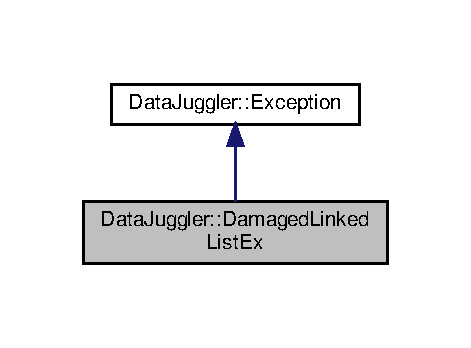
\includegraphics[width=226pt]{classDataJuggler_1_1DamagedLinkedListEx__inherit__graph}
\end{center}
\end{figure}


Collaboration diagram for Data\+Juggler\+:\+:Damaged\+Linked\+List\+Ex\+:\nopagebreak
\begin{figure}[H]
\begin{center}
\leavevmode
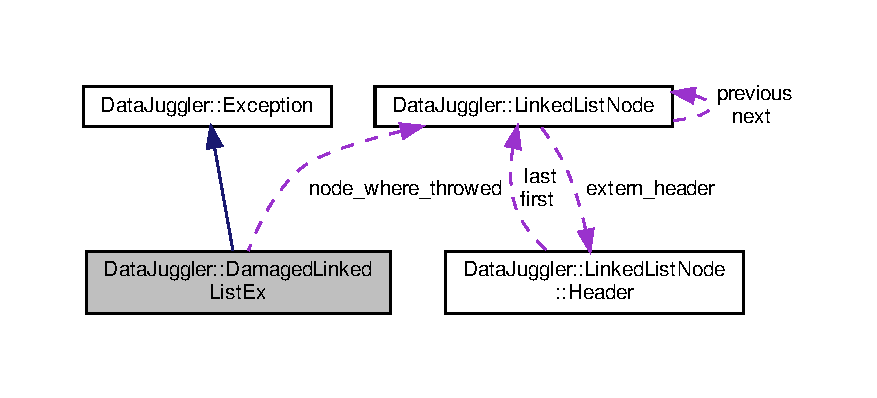
\includegraphics[width=350pt]{classDataJuggler_1_1DamagedLinkedListEx__coll__graph}
\end{center}
\end{figure}
\subsection*{Public Member Functions}
\begin{DoxyCompactItemize}
\item 
\mbox{\Hypertarget{classDataJuggler_1_1DamagedLinkedListEx_a07957e3a7722d5d7adf90bf013786de8}\label{classDataJuggler_1_1DamagedLinkedListEx_a07957e3a7722d5d7adf90bf013786de8}} 
{\bfseries Damaged\+Linked\+List\+Ex} (\hyperlink{classDataJuggler_1_1LinkedListNode}{Linked\+List\+Node} $\ast$node\+\_\+where\+\_\+throwed)
\end{DoxyCompactItemize}
\subsection*{Public Attributes}
\begin{DoxyCompactItemize}
\item 
\mbox{\Hypertarget{classDataJuggler_1_1DamagedLinkedListEx_afd9cb052b1989a06612862adef82eeb6}\label{classDataJuggler_1_1DamagedLinkedListEx_afd9cb052b1989a06612862adef82eeb6}} 
\hyperlink{classDataJuggler_1_1LinkedListNode}{Linked\+List\+Node} $\ast$ {\bfseries node\+\_\+where\+\_\+throwed}
\end{DoxyCompactItemize}
\subsection*{Static Public Attributes}
\begin{DoxyCompactItemize}
\item 
\mbox{\Hypertarget{classDataJuggler_1_1DamagedLinkedListEx_abb7d42fefb001c0e6370ae703bee976e}\label{classDataJuggler_1_1DamagedLinkedListEx_abb7d42fefb001c0e6370ae703bee976e}} 
static const unsigned long long {\bfseries default\+Code} = 11246
\end{DoxyCompactItemize}


\subsection{Detailed Description}
This class represents an exception caused by a logical error in a linked list. When a logical error is detected in the linked list, this class is instantiated and an exception is thrown with it. 

The documentation for this class was generated from the following files\+:\begin{DoxyCompactItemize}
\item 
src/linearnode.\+hpp\item 
src/linearnode.\+cpp\end{DoxyCompactItemize}

\hypertarget{classDataJuggler_1_1Exception}{}\section{Data\+Juggler\+:\+:Exception Class Reference}
\label{classDataJuggler_1_1Exception}\index{Data\+Juggler\+::\+Exception@{Data\+Juggler\+::\+Exception}}


Inheritance diagram for Data\+Juggler\+:\+:Exception\+:\nopagebreak
\begin{figure}[H]
\begin{center}
\leavevmode
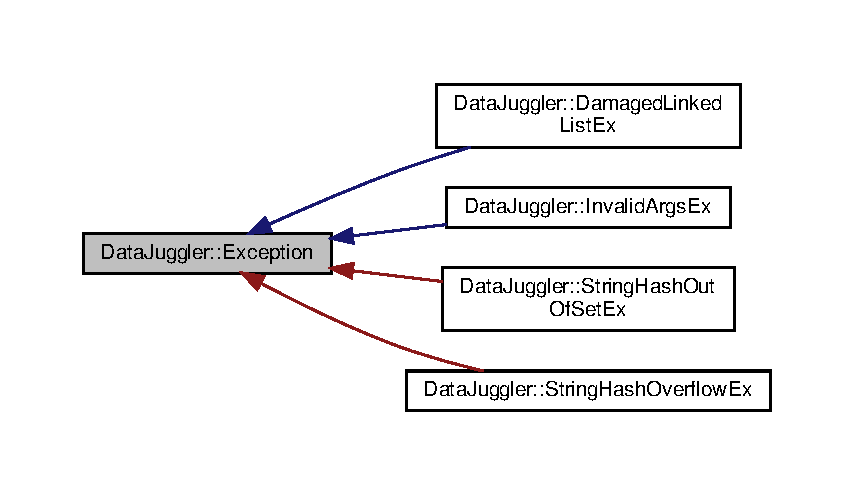
\includegraphics[width=350pt]{classDataJuggler_1_1Exception__inherit__graph}
\end{center}
\end{figure}
\subsection*{Public Member Functions}
\begin{DoxyCompactItemize}
\item 
\mbox{\Hypertarget{classDataJuggler_1_1Exception_ac61ec302c994b32c99218c005fa2d632}\label{classDataJuggler_1_1Exception_ac61ec302c994b32c99218c005fa2d632}} 
{\bfseries Exception} (unsigned long long code, string name, string description)
\end{DoxyCompactItemize}
\subsection*{Public Attributes}
\begin{DoxyCompactItemize}
\item 
\mbox{\Hypertarget{classDataJuggler_1_1Exception_a6b96bbed8c31affc3976a568a5dbccff}\label{classDataJuggler_1_1Exception_a6b96bbed8c31affc3976a568a5dbccff}} 
unsigned long long {\bfseries code}
\item 
\mbox{\Hypertarget{classDataJuggler_1_1Exception_ac309e75d14836ba5edfec506658432e6}\label{classDataJuggler_1_1Exception_ac309e75d14836ba5edfec506658432e6}} 
string {\bfseries name}
\item 
\mbox{\Hypertarget{classDataJuggler_1_1Exception_a29fc76f45d57d2ddf4b92657f491f694}\label{classDataJuggler_1_1Exception_a29fc76f45d57d2ddf4b92657f491f694}} 
string {\bfseries description}
\end{DoxyCompactItemize}


The documentation for this class was generated from the following files\+:\begin{DoxyCompactItemize}
\item 
src/exception.\+hpp\item 
src/exception.\+cpp\end{DoxyCompactItemize}

\hypertarget{classDataJuggler_1_1LinkedListNode_1_1Header}{}\section{Data\+Juggler\+:\+:Linked\+List\+Node\+:\+:Header Class Reference}
\label{classDataJuggler_1_1LinkedListNode_1_1Header}\index{Data\+Juggler\+::\+Linked\+List\+Node\+::\+Header@{Data\+Juggler\+::\+Linked\+List\+Node\+::\+Header}}


{\ttfamily \#include $<$linearnode.\+hpp$>$}



Collaboration diagram for Data\+Juggler\+:\+:Linked\+List\+Node\+:\+:Header\+:\nopagebreak
\begin{figure}[H]
\begin{center}
\leavevmode
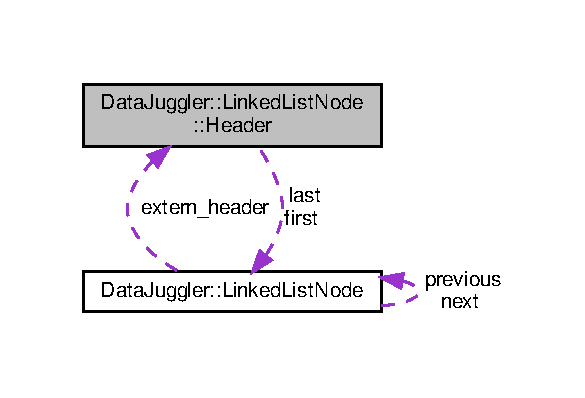
\includegraphics[width=281pt]{classDataJuggler_1_1LinkedListNode_1_1Header__coll__graph}
\end{center}
\end{figure}
\subsection*{Public Attributes}
\begin{DoxyCompactItemize}
\item 
\mbox{\Hypertarget{classDataJuggler_1_1LinkedListNode_1_1Header_a6d97ef022c673321ce13867e3c1d5b17}\label{classDataJuggler_1_1LinkedListNode_1_1Header_a6d97ef022c673321ce13867e3c1d5b17}} 
unsigned long {\bfseries counter}
\item 
\mbox{\Hypertarget{classDataJuggler_1_1LinkedListNode_1_1Header_abe505da1ec81b359371c0aa4631a01f2}\label{classDataJuggler_1_1LinkedListNode_1_1Header_abe505da1ec81b359371c0aa4631a01f2}} 
\hyperlink{classDataJuggler_1_1LinkedListNode}{Linked\+List\+Node} $\ast$ {\bfseries first}
\item 
\mbox{\Hypertarget{classDataJuggler_1_1LinkedListNode_1_1Header_ad81659985a9776933338bc6f2b730e80}\label{classDataJuggler_1_1LinkedListNode_1_1Header_ad81659985a9776933338bc6f2b730e80}} 
\hyperlink{classDataJuggler_1_1LinkedListNode}{Linked\+List\+Node} $\ast$ {\bfseries last}
\end{DoxyCompactItemize}


\subsection{Detailed Description}
This class represents the header of a list formed by Linked\+List\+Nodes. 

The documentation for this class was generated from the following file\+:\begin{DoxyCompactItemize}
\item 
src/linearnode.\+hpp\end{DoxyCompactItemize}

\hypertarget{classDataJuggler_1_1InvalidArgsEx}{}\section{Data\+Juggler\+:\+:Invalid\+Args\+Ex Class Reference}
\label{classDataJuggler_1_1InvalidArgsEx}\index{Data\+Juggler\+::\+Invalid\+Args\+Ex@{Data\+Juggler\+::\+Invalid\+Args\+Ex}}


Inheritance diagram for Data\+Juggler\+:\+:Invalid\+Args\+Ex\+:\nopagebreak
\begin{figure}[H]
\begin{center}
\leavevmode
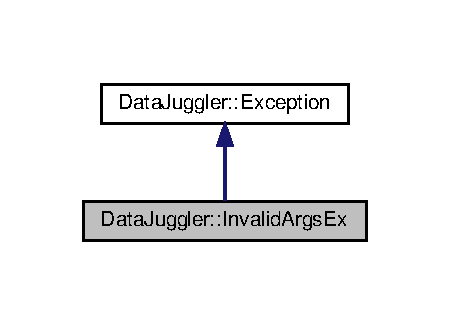
\includegraphics[width=216pt]{classDataJuggler_1_1InvalidArgsEx__inherit__graph}
\end{center}
\end{figure}


Collaboration diagram for Data\+Juggler\+:\+:Invalid\+Args\+Ex\+:\nopagebreak
\begin{figure}[H]
\begin{center}
\leavevmode
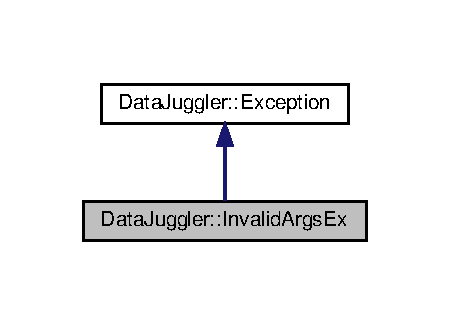
\includegraphics[width=216pt]{classDataJuggler_1_1InvalidArgsEx__coll__graph}
\end{center}
\end{figure}
\subsection*{Public Member Functions}
\begin{DoxyCompactItemize}
\item 
\mbox{\Hypertarget{classDataJuggler_1_1InvalidArgsEx_a5ab92559ef9ee96508fa766075e9d80d}\label{classDataJuggler_1_1InvalidArgsEx_a5ab92559ef9ee96508fa766075e9d80d}} 
{\bfseries Invalid\+Args\+Ex} (string function\+\_\+name, string param\+\_\+name)
\end{DoxyCompactItemize}
\subsection*{Public Attributes}
\begin{DoxyCompactItemize}
\item 
\mbox{\Hypertarget{classDataJuggler_1_1InvalidArgsEx_ae5cf96c161a746440d9020a1e08ea064}\label{classDataJuggler_1_1InvalidArgsEx_ae5cf96c161a746440d9020a1e08ea064}} 
string {\bfseries function\+\_\+name}
\item 
\mbox{\Hypertarget{classDataJuggler_1_1InvalidArgsEx_abae3048ec919313a22f58a5787e55c6f}\label{classDataJuggler_1_1InvalidArgsEx_abae3048ec919313a22f58a5787e55c6f}} 
string {\bfseries param\+\_\+name}
\end{DoxyCompactItemize}
\subsection*{Static Public Attributes}
\begin{DoxyCompactItemize}
\item 
\mbox{\Hypertarget{classDataJuggler_1_1InvalidArgsEx_a89a2a9b6d4da8c42d1d5511a4bc66890}\label{classDataJuggler_1_1InvalidArgsEx_a89a2a9b6d4da8c42d1d5511a4bc66890}} 
static const unsigned long long {\bfseries default\+Code} = 5267
\end{DoxyCompactItemize}


The documentation for this class was generated from the following files\+:\begin{DoxyCompactItemize}
\item 
src/exception.\+hpp\item 
src/exception.\+cpp\end{DoxyCompactItemize}

\hypertarget{classDataJuggler_1_1LinkedListNode}{}\section{Data\+Juggler\+:\+:Linked\+List\+Node Class Reference}
\label{classDataJuggler_1_1LinkedListNode}\index{Data\+Juggler\+::\+Linked\+List\+Node@{Data\+Juggler\+::\+Linked\+List\+Node}}


{\ttfamily \#include $<$linearnode.\+hpp$>$}



Collaboration diagram for Data\+Juggler\+:\+:Linked\+List\+Node\+:\nopagebreak
\begin{figure}[H]
\begin{center}
\leavevmode
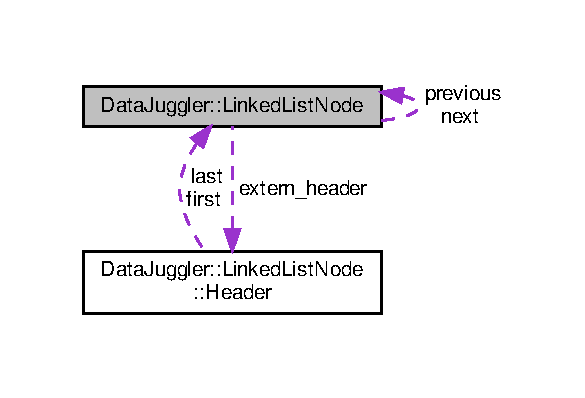
\includegraphics[width=281pt]{classDataJuggler_1_1LinkedListNode__coll__graph}
\end{center}
\end{figure}
\subsection*{Classes}
\begin{DoxyCompactItemize}
\item 
class \hyperlink{classDataJuggler_1_1LinkedListNode_1_1Header}{Header}
\end{DoxyCompactItemize}
\subsection*{Public Member Functions}
\begin{DoxyCompactItemize}
\item 
\hyperlink{classDataJuggler_1_1LinkedListNode_af152a8cc8a324734b8aaaf59736ccec1}{Linked\+List\+Node} (\hyperlink{classDataJuggler_1_1LinkedListNode_1_1Header}{Linked\+List\+Node\+::\+Header} $\ast$extern\+\_\+header)
\item 
\hyperlink{classDataJuggler_1_1LinkedListNode_a5791a156ded0c87075b8add6d18c0d51}{Linked\+List\+Node} (\hyperlink{classDataJuggler_1_1LinkedListNode_1_1Header}{Linked\+List\+Node\+::\+Header} \&extern\+\_\+header)
\item 
virtual void \hyperlink{classDataJuggler_1_1LinkedListNode_ae3a9bfcf7f4b13dd0d1f3095626aa108}{Clone\+From} (\hyperlink{classDataJuggler_1_1LinkedListNode}{Linked\+List\+Node} $\ast$to\+\_\+copy)
\item 
virtual void \hyperlink{classDataJuggler_1_1LinkedListNode_ad508fe0c993b16caf5a627e1f265754b}{Clone\+From} (\hyperlink{classDataJuggler_1_1LinkedListNode}{Linked\+List\+Node} \&to\+\_\+copy)
\item 
void \hyperlink{classDataJuggler_1_1LinkedListNode_a509b4493bb13fc771481da50f7593bd9}{insert\+After} (\hyperlink{classDataJuggler_1_1LinkedListNode}{Linked\+List\+Node} $\ast$to\+\_\+insert)
\item 
void \hyperlink{classDataJuggler_1_1LinkedListNode_a50f738d5f3c69e78f417ab5172924a8c}{insert\+Before} (\hyperlink{classDataJuggler_1_1LinkedListNode}{Linked\+List\+Node} $\ast$to\+\_\+insert)
\item 
void \hyperlink{classDataJuggler_1_1LinkedListNode_a007fd147dbf3ca2d83a7c40d5181c26c}{remove} ()
\item 
void \hyperlink{classDataJuggler_1_1LinkedListNode_ad4166bef988c213884d2dc5962519bbb}{move\+To\+After\+Of} (\hyperlink{classDataJuggler_1_1LinkedListNode}{Linked\+List\+Node} $\ast$ref\+\_\+node)
\item 
void \hyperlink{classDataJuggler_1_1LinkedListNode_a88c44bb0d302955fa4be2b1d5e1c743b}{move\+To\+Before\+Of} (\hyperlink{classDataJuggler_1_1LinkedListNode}{Linked\+List\+Node} $\ast$ref\+\_\+node)
\item 
\hyperlink{classDataJuggler_1_1LinkedListNode}{Linked\+List\+Node} $\ast$ \hyperlink{classDataJuggler_1_1LinkedListNode_a65f28eec41e48b46fe28579ef029da16}{get\+Next} ()
\item 
\hyperlink{classDataJuggler_1_1LinkedListNode}{Linked\+List\+Node} $\ast$ \hyperlink{classDataJuggler_1_1LinkedListNode_a12df61829bc55f904a6c7e3c71ab0cdd}{get\+Previous} ()
\item 
void \hyperlink{classDataJuggler_1_1LinkedListNode_ac178b6c57266b64be44d3b7aff54e6b8}{check\+Integrity} ()
\end{DoxyCompactItemize}
\subsection*{Protected Attributes}
\begin{DoxyCompactItemize}
\item 
\mbox{\Hypertarget{classDataJuggler_1_1LinkedListNode_a614e5c1d3c3fe2821eb64429e0cfbf8b}\label{classDataJuggler_1_1LinkedListNode_a614e5c1d3c3fe2821eb64429e0cfbf8b}} 
\hyperlink{classDataJuggler_1_1LinkedListNode_1_1Header}{Linked\+List\+Node\+::\+Header} $\ast$ {\bfseries extern\+\_\+header}
\item 
\mbox{\Hypertarget{classDataJuggler_1_1LinkedListNode_a555e08ab7b31e45dbf32e0cb5b3edfd1}\label{classDataJuggler_1_1LinkedListNode_a555e08ab7b31e45dbf32e0cb5b3edfd1}} 
\hyperlink{classDataJuggler_1_1LinkedListNode}{Linked\+List\+Node} $\ast$ {\bfseries next}
\item 
\mbox{\Hypertarget{classDataJuggler_1_1LinkedListNode_a60ebbf55f9b6c6bd2932c929ce7a2f26}\label{classDataJuggler_1_1LinkedListNode_a60ebbf55f9b6c6bd2932c929ce7a2f26}} 
\hyperlink{classDataJuggler_1_1LinkedListNode}{Linked\+List\+Node} $\ast$ {\bfseries previous}
\end{DoxyCompactItemize}


\subsection{Detailed Description}
This class represents the double-\/linked node of a list structure. This class is basic and should not be instantiated directly. Subclasses of this can be used to insert data into the node. 

\subsection{Constructor \& Destructor Documentation}
\mbox{\Hypertarget{classDataJuggler_1_1LinkedListNode_af152a8cc8a324734b8aaaf59736ccec1}\label{classDataJuggler_1_1LinkedListNode_af152a8cc8a324734b8aaaf59736ccec1}} 
\index{Data\+Juggler\+::\+Linked\+List\+Node@{Data\+Juggler\+::\+Linked\+List\+Node}!Linked\+List\+Node@{Linked\+List\+Node}}
\index{Linked\+List\+Node@{Linked\+List\+Node}!Data\+Juggler\+::\+Linked\+List\+Node@{Data\+Juggler\+::\+Linked\+List\+Node}}
\subsubsection{\texorpdfstring{Linked\+List\+Node()}{LinkedListNode()}\hspace{0.1cm}{\footnotesize\ttfamily [1/2]}}
{\footnotesize\ttfamily Data\+Juggler\+::\+Linked\+List\+Node\+::\+Linked\+List\+Node (\begin{DoxyParamCaption}\item[{\hyperlink{classDataJuggler_1_1LinkedListNode_1_1Header}{Linked\+List\+Node\+::\+Header} $\ast$}]{extern\+\_\+header }\end{DoxyParamCaption})}

This constructor takes as an argument a pointer to the list header \mbox{\Hypertarget{classDataJuggler_1_1LinkedListNode_a5791a156ded0c87075b8add6d18c0d51}\label{classDataJuggler_1_1LinkedListNode_a5791a156ded0c87075b8add6d18c0d51}} 
\index{Data\+Juggler\+::\+Linked\+List\+Node@{Data\+Juggler\+::\+Linked\+List\+Node}!Linked\+List\+Node@{Linked\+List\+Node}}
\index{Linked\+List\+Node@{Linked\+List\+Node}!Data\+Juggler\+::\+Linked\+List\+Node@{Data\+Juggler\+::\+Linked\+List\+Node}}
\subsubsection{\texorpdfstring{Linked\+List\+Node()}{LinkedListNode()}\hspace{0.1cm}{\footnotesize\ttfamily [2/2]}}
{\footnotesize\ttfamily Data\+Juggler\+::\+Linked\+List\+Node\+::\+Linked\+List\+Node (\begin{DoxyParamCaption}\item[{\hyperlink{classDataJuggler_1_1LinkedListNode_1_1Header}{Linked\+List\+Node\+::\+Header} \&}]{extern\+\_\+header }\end{DoxyParamCaption})}

This constructor takes as an argument a reference to the list header 

\subsection{Member Function Documentation}
\mbox{\Hypertarget{classDataJuggler_1_1LinkedListNode_ac178b6c57266b64be44d3b7aff54e6b8}\label{classDataJuggler_1_1LinkedListNode_ac178b6c57266b64be44d3b7aff54e6b8}} 
\index{Data\+Juggler\+::\+Linked\+List\+Node@{Data\+Juggler\+::\+Linked\+List\+Node}!check\+Integrity@{check\+Integrity}}
\index{check\+Integrity@{check\+Integrity}!Data\+Juggler\+::\+Linked\+List\+Node@{Data\+Juggler\+::\+Linked\+List\+Node}}
\subsubsection{\texorpdfstring{check\+Integrity()}{checkIntegrity()}}
{\footnotesize\ttfamily void Data\+Juggler\+::\+Linked\+List\+Node\+::check\+Integrity (\begin{DoxyParamCaption}{ }\end{DoxyParamCaption})}

Checks for logical errors in the linked list \mbox{\Hypertarget{classDataJuggler_1_1LinkedListNode_ae3a9bfcf7f4b13dd0d1f3095626aa108}\label{classDataJuggler_1_1LinkedListNode_ae3a9bfcf7f4b13dd0d1f3095626aa108}} 
\index{Data\+Juggler\+::\+Linked\+List\+Node@{Data\+Juggler\+::\+Linked\+List\+Node}!Clone\+From@{Clone\+From}}
\index{Clone\+From@{Clone\+From}!Data\+Juggler\+::\+Linked\+List\+Node@{Data\+Juggler\+::\+Linked\+List\+Node}}
\subsubsection{\texorpdfstring{Clone\+From()}{CloneFrom()}\hspace{0.1cm}{\footnotesize\ttfamily [1/2]}}
{\footnotesize\ttfamily void Data\+Juggler\+::\+Linked\+List\+Node\+::\+Clone\+From (\begin{DoxyParamCaption}\item[{\hyperlink{classDataJuggler_1_1LinkedListNode}{Linked\+List\+Node} $\ast$}]{to\+\_\+copy }\end{DoxyParamCaption})\hspace{0.3cm}{\ttfamily [virtual]}}

Make it a copy of another \hyperlink{classDataJuggler_1_1LinkedListNode}{Linked\+List\+Node} (object from pointer) \mbox{\Hypertarget{classDataJuggler_1_1LinkedListNode_ad508fe0c993b16caf5a627e1f265754b}\label{classDataJuggler_1_1LinkedListNode_ad508fe0c993b16caf5a627e1f265754b}} 
\index{Data\+Juggler\+::\+Linked\+List\+Node@{Data\+Juggler\+::\+Linked\+List\+Node}!Clone\+From@{Clone\+From}}
\index{Clone\+From@{Clone\+From}!Data\+Juggler\+::\+Linked\+List\+Node@{Data\+Juggler\+::\+Linked\+List\+Node}}
\subsubsection{\texorpdfstring{Clone\+From()}{CloneFrom()}\hspace{0.1cm}{\footnotesize\ttfamily [2/2]}}
{\footnotesize\ttfamily void Data\+Juggler\+::\+Linked\+List\+Node\+::\+Clone\+From (\begin{DoxyParamCaption}\item[{\hyperlink{classDataJuggler_1_1LinkedListNode}{Linked\+List\+Node} \&}]{to\+\_\+copy }\end{DoxyParamCaption})\hspace{0.3cm}{\ttfamily [virtual]}}

Make it a copy of another \hyperlink{classDataJuggler_1_1LinkedListNode}{Linked\+List\+Node} (object from reference) \mbox{\Hypertarget{classDataJuggler_1_1LinkedListNode_a65f28eec41e48b46fe28579ef029da16}\label{classDataJuggler_1_1LinkedListNode_a65f28eec41e48b46fe28579ef029da16}} 
\index{Data\+Juggler\+::\+Linked\+List\+Node@{Data\+Juggler\+::\+Linked\+List\+Node}!get\+Next@{get\+Next}}
\index{get\+Next@{get\+Next}!Data\+Juggler\+::\+Linked\+List\+Node@{Data\+Juggler\+::\+Linked\+List\+Node}}
\subsubsection{\texorpdfstring{get\+Next()}{getNext()}}
{\footnotesize\ttfamily \hyperlink{classDataJuggler_1_1LinkedListNode}{Linked\+List\+Node} $\ast$ Data\+Juggler\+::\+Linked\+List\+Node\+::get\+Next (\begin{DoxyParamCaption}{ }\end{DoxyParamCaption})}

Get the next node of this in the list \mbox{\Hypertarget{classDataJuggler_1_1LinkedListNode_a12df61829bc55f904a6c7e3c71ab0cdd}\label{classDataJuggler_1_1LinkedListNode_a12df61829bc55f904a6c7e3c71ab0cdd}} 
\index{Data\+Juggler\+::\+Linked\+List\+Node@{Data\+Juggler\+::\+Linked\+List\+Node}!get\+Previous@{get\+Previous}}
\index{get\+Previous@{get\+Previous}!Data\+Juggler\+::\+Linked\+List\+Node@{Data\+Juggler\+::\+Linked\+List\+Node}}
\subsubsection{\texorpdfstring{get\+Previous()}{getPrevious()}}
{\footnotesize\ttfamily \hyperlink{classDataJuggler_1_1LinkedListNode}{Linked\+List\+Node} $\ast$ Data\+Juggler\+::\+Linked\+List\+Node\+::get\+Previous (\begin{DoxyParamCaption}{ }\end{DoxyParamCaption})}

Get the previous node of this in the list \mbox{\Hypertarget{classDataJuggler_1_1LinkedListNode_a509b4493bb13fc771481da50f7593bd9}\label{classDataJuggler_1_1LinkedListNode_a509b4493bb13fc771481da50f7593bd9}} 
\index{Data\+Juggler\+::\+Linked\+List\+Node@{Data\+Juggler\+::\+Linked\+List\+Node}!insert\+After@{insert\+After}}
\index{insert\+After@{insert\+After}!Data\+Juggler\+::\+Linked\+List\+Node@{Data\+Juggler\+::\+Linked\+List\+Node}}
\subsubsection{\texorpdfstring{insert\+After()}{insertAfter()}}
{\footnotesize\ttfamily void Data\+Juggler\+::\+Linked\+List\+Node\+::insert\+After (\begin{DoxyParamCaption}\item[{\hyperlink{classDataJuggler_1_1LinkedListNode}{Linked\+List\+Node} $\ast$}]{to\+\_\+insert }\end{DoxyParamCaption})}

Insert a node after this in linked list \mbox{\Hypertarget{classDataJuggler_1_1LinkedListNode_a50f738d5f3c69e78f417ab5172924a8c}\label{classDataJuggler_1_1LinkedListNode_a50f738d5f3c69e78f417ab5172924a8c}} 
\index{Data\+Juggler\+::\+Linked\+List\+Node@{Data\+Juggler\+::\+Linked\+List\+Node}!insert\+Before@{insert\+Before}}
\index{insert\+Before@{insert\+Before}!Data\+Juggler\+::\+Linked\+List\+Node@{Data\+Juggler\+::\+Linked\+List\+Node}}
\subsubsection{\texorpdfstring{insert\+Before()}{insertBefore()}}
{\footnotesize\ttfamily void Data\+Juggler\+::\+Linked\+List\+Node\+::insert\+Before (\begin{DoxyParamCaption}\item[{\hyperlink{classDataJuggler_1_1LinkedListNode}{Linked\+List\+Node} $\ast$}]{to\+\_\+insert }\end{DoxyParamCaption})}

Insert a node before this in linked list \mbox{\Hypertarget{classDataJuggler_1_1LinkedListNode_ad4166bef988c213884d2dc5962519bbb}\label{classDataJuggler_1_1LinkedListNode_ad4166bef988c213884d2dc5962519bbb}} 
\index{Data\+Juggler\+::\+Linked\+List\+Node@{Data\+Juggler\+::\+Linked\+List\+Node}!move\+To\+After\+Of@{move\+To\+After\+Of}}
\index{move\+To\+After\+Of@{move\+To\+After\+Of}!Data\+Juggler\+::\+Linked\+List\+Node@{Data\+Juggler\+::\+Linked\+List\+Node}}
\subsubsection{\texorpdfstring{move\+To\+After\+Of()}{moveToAfterOf()}}
{\footnotesize\ttfamily void Data\+Juggler\+::\+Linked\+List\+Node\+::move\+To\+After\+Of (\begin{DoxyParamCaption}\item[{\hyperlink{classDataJuggler_1_1LinkedListNode}{Linked\+List\+Node} $\ast$}]{ref\+\_\+node }\end{DoxyParamCaption})}

Move this node to after of a reference node of the same list \mbox{\Hypertarget{classDataJuggler_1_1LinkedListNode_a88c44bb0d302955fa4be2b1d5e1c743b}\label{classDataJuggler_1_1LinkedListNode_a88c44bb0d302955fa4be2b1d5e1c743b}} 
\index{Data\+Juggler\+::\+Linked\+List\+Node@{Data\+Juggler\+::\+Linked\+List\+Node}!move\+To\+Before\+Of@{move\+To\+Before\+Of}}
\index{move\+To\+Before\+Of@{move\+To\+Before\+Of}!Data\+Juggler\+::\+Linked\+List\+Node@{Data\+Juggler\+::\+Linked\+List\+Node}}
\subsubsection{\texorpdfstring{move\+To\+Before\+Of()}{moveToBeforeOf()}}
{\footnotesize\ttfamily void Data\+Juggler\+::\+Linked\+List\+Node\+::move\+To\+Before\+Of (\begin{DoxyParamCaption}\item[{\hyperlink{classDataJuggler_1_1LinkedListNode}{Linked\+List\+Node} $\ast$}]{ref\+\_\+node }\end{DoxyParamCaption})}

Move this node to before of a reference node of the same list \mbox{\Hypertarget{classDataJuggler_1_1LinkedListNode_a007fd147dbf3ca2d83a7c40d5181c26c}\label{classDataJuggler_1_1LinkedListNode_a007fd147dbf3ca2d83a7c40d5181c26c}} 
\index{Data\+Juggler\+::\+Linked\+List\+Node@{Data\+Juggler\+::\+Linked\+List\+Node}!remove@{remove}}
\index{remove@{remove}!Data\+Juggler\+::\+Linked\+List\+Node@{Data\+Juggler\+::\+Linked\+List\+Node}}
\subsubsection{\texorpdfstring{remove()}{remove()}}
{\footnotesize\ttfamily void Data\+Juggler\+::\+Linked\+List\+Node\+::remove (\begin{DoxyParamCaption}{ }\end{DoxyParamCaption})}

Remove this node from the linked list (without delete this) 

The documentation for this class was generated from the following files\+:\begin{DoxyCompactItemize}
\item 
src/linearnode.\+hpp\item 
src/linearnode.\+cpp\end{DoxyCompactItemize}

\hypertarget{classDataJuggler_1_1StringHashOutOfSetEx}{}\section{Data\+Juggler\+:\+:String\+Hash\+Out\+Of\+Set\+Ex Class Reference}
\label{classDataJuggler_1_1StringHashOutOfSetEx}\index{Data\+Juggler\+::\+String\+Hash\+Out\+Of\+Set\+Ex@{Data\+Juggler\+::\+String\+Hash\+Out\+Of\+Set\+Ex}}


Inheritance diagram for Data\+Juggler\+:\+:String\+Hash\+Out\+Of\+Set\+Ex\+:\nopagebreak
\begin{figure}[H]
\begin{center}
\leavevmode
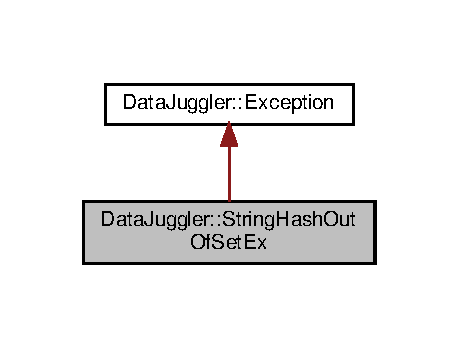
\includegraphics[width=220pt]{classDataJuggler_1_1StringHashOutOfSetEx__inherit__graph}
\end{center}
\end{figure}


Collaboration diagram for Data\+Juggler\+:\+:String\+Hash\+Out\+Of\+Set\+Ex\+:\nopagebreak
\begin{figure}[H]
\begin{center}
\leavevmode
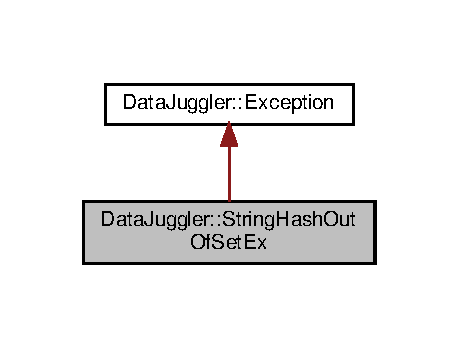
\includegraphics[width=220pt]{classDataJuggler_1_1StringHashOutOfSetEx__coll__graph}
\end{center}
\end{figure}
\subsection*{Public Member Functions}
\begin{DoxyCompactItemize}
\item 
\mbox{\Hypertarget{classDataJuggler_1_1StringHashOutOfSetEx_a47bfc18b15192c219a737aa54dbc3dd1}\label{classDataJuggler_1_1StringHashOutOfSetEx_a47bfc18b15192c219a737aa54dbc3dd1}} 
{\bfseries String\+Hash\+Out\+Of\+Set\+Ex} (string guilty, string charset, unsigned long guilty\+\_\+char\+\_\+index)
\end{DoxyCompactItemize}
\subsection*{Public Attributes}
\begin{DoxyCompactItemize}
\item 
\mbox{\Hypertarget{classDataJuggler_1_1StringHashOutOfSetEx_aa5c313e22f91e09002e3bb3f8f866db9}\label{classDataJuggler_1_1StringHashOutOfSetEx_aa5c313e22f91e09002e3bb3f8f866db9}} 
string {\bfseries guilty}
\item 
\mbox{\Hypertarget{classDataJuggler_1_1StringHashOutOfSetEx_ac99fb53369b60fa66bc0d26b7ef6bcf5}\label{classDataJuggler_1_1StringHashOutOfSetEx_ac99fb53369b60fa66bc0d26b7ef6bcf5}} 
string {\bfseries charset}
\item 
\mbox{\Hypertarget{classDataJuggler_1_1StringHashOutOfSetEx_a4ab18c72c3690d809bcc1d9d69589348}\label{classDataJuggler_1_1StringHashOutOfSetEx_a4ab18c72c3690d809bcc1d9d69589348}} 
unsigned long {\bfseries guilty\+\_\+char\+\_\+index}
\end{DoxyCompactItemize}
\subsection*{Static Public Attributes}
\begin{DoxyCompactItemize}
\item 
\mbox{\Hypertarget{classDataJuggler_1_1StringHashOutOfSetEx_a719d3f8abab813f822c91804e0f76030}\label{classDataJuggler_1_1StringHashOutOfSetEx_a719d3f8abab813f822c91804e0f76030}} 
static const unsigned long long {\bfseries default\+Code} = 12599
\end{DoxyCompactItemize}


The documentation for this class was generated from the following files\+:\begin{DoxyCompactItemize}
\item 
src/stringhash.\+hpp\item 
src/stringhash.\+cpp\end{DoxyCompactItemize}

\hypertarget{classDataJuggler_1_1StringHashOverflowEx}{}\section{Data\+Juggler\+:\+:String\+Hash\+Overflow\+Ex Class Reference}
\label{classDataJuggler_1_1StringHashOverflowEx}\index{Data\+Juggler\+::\+String\+Hash\+Overflow\+Ex@{Data\+Juggler\+::\+String\+Hash\+Overflow\+Ex}}


Inheritance diagram for Data\+Juggler\+:\+:String\+Hash\+Overflow\+Ex\+:\nopagebreak
\begin{figure}[H]
\begin{center}
\leavevmode
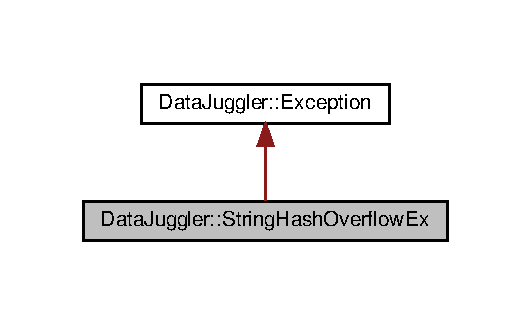
\includegraphics[width=255pt]{classDataJuggler_1_1StringHashOverflowEx__inherit__graph}
\end{center}
\end{figure}


Collaboration diagram for Data\+Juggler\+:\+:String\+Hash\+Overflow\+Ex\+:\nopagebreak
\begin{figure}[H]
\begin{center}
\leavevmode
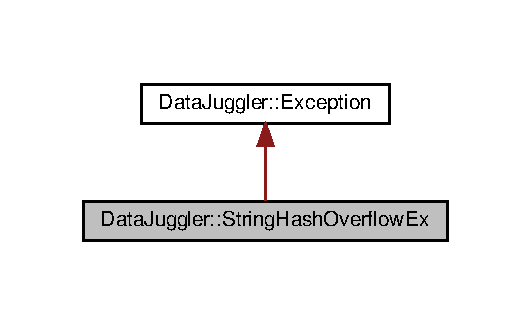
\includegraphics[width=255pt]{classDataJuggler_1_1StringHashOverflowEx__coll__graph}
\end{center}
\end{figure}
\subsection*{Public Member Functions}
\begin{DoxyCompactItemize}
\item 
\mbox{\Hypertarget{classDataJuggler_1_1StringHashOverflowEx_a1b015bde7404e9de2b790d3ced167488}\label{classDataJuggler_1_1StringHashOverflowEx_a1b015bde7404e9de2b790d3ced167488}} 
{\bfseries String\+Hash\+Overflow\+Ex} (string guilty)
\end{DoxyCompactItemize}
\subsection*{Public Attributes}
\begin{DoxyCompactItemize}
\item 
\mbox{\Hypertarget{classDataJuggler_1_1StringHashOverflowEx_aa1eacc7cf8dfaf161bc8287882b886d8}\label{classDataJuggler_1_1StringHashOverflowEx_aa1eacc7cf8dfaf161bc8287882b886d8}} 
string {\bfseries guilty}
\end{DoxyCompactItemize}
\subsection*{Static Public Attributes}
\begin{DoxyCompactItemize}
\item 
\mbox{\Hypertarget{classDataJuggler_1_1StringHashOverflowEx_a8ccbc125218a45e4782d4e2379eae332}\label{classDataJuggler_1_1StringHashOverflowEx_a8ccbc125218a45e4782d4e2379eae332}} 
static const unsigned long long {\bfseries default\+Code} = 12542
\end{DoxyCompactItemize}


The documentation for this class was generated from the following files\+:\begin{DoxyCompactItemize}
\item 
src/stringhash.\+hpp\item 
src/stringhash.\+cpp\end{DoxyCompactItemize}

%--- End generated contents ---

% Index
\backmatter
\newpage
\phantomsection
\clearemptydoublepage
\addcontentsline{toc}{chapter}{Index}
\printindex

\end{document}
